\section{Design Patterns} \label{designpatterns}

\subsection{Description}

\noindent\fbox{
	\parbox{\textwidth}{
		\textbf{4.} Design the software and apply design patterns that are suitable for your project, and motivate the choice of the used patterns. Use the Two-Part Architecture Model if relevant for the problem. Use the abstract OS package for the ZYBO board.
	}
}\citepawesome{Bjerge2017}{1}

In the following solution the patterns \citeawesome{RalphJohnsonErichGammaJohnVlissides}  used are:
\begin{itemize}
	\item State Pattern
	\item Singleton
	\item Command Pattern
\end{itemize}

In this project it made sense to implement the State Pattern, Singletons and Command Pattern. Each of the patterens is covered in the sections below.

\subsection{GOF State Pattern}
The intent of the state pattern is to grant an object the ability to change its behavior when it's internal state changes hence the object will therefore change its class. Consider a the state machine digram in figure \ref{fig:smdguistate} that represents the gui of the PSOS. The PSOS can be in one of the distinct states: Setup, FindMinima, FindMaxima. \\

When the Zynq CPU starts we enter the Setup state. This receives actions from other classes such as ActionUp, ActionDown, ActionNext and it's responds will differ base on the action. For example, the result of an StartAction depends on what the current state is in, the FindMinima or FindMaxima state can both use it, but the setup does not accept it. The choice to include the GOF State Pattern was made because it is a easy way to model an existing state machine from a digram into fully working software. \\

As seen in Figure \ref{fig:statemachine}, is the state machine in the project. It was a good choice to use the GOF State Pattern because of the ease to model a state machine and bring it into code. 

\begin{figure}[h]
	\centering
	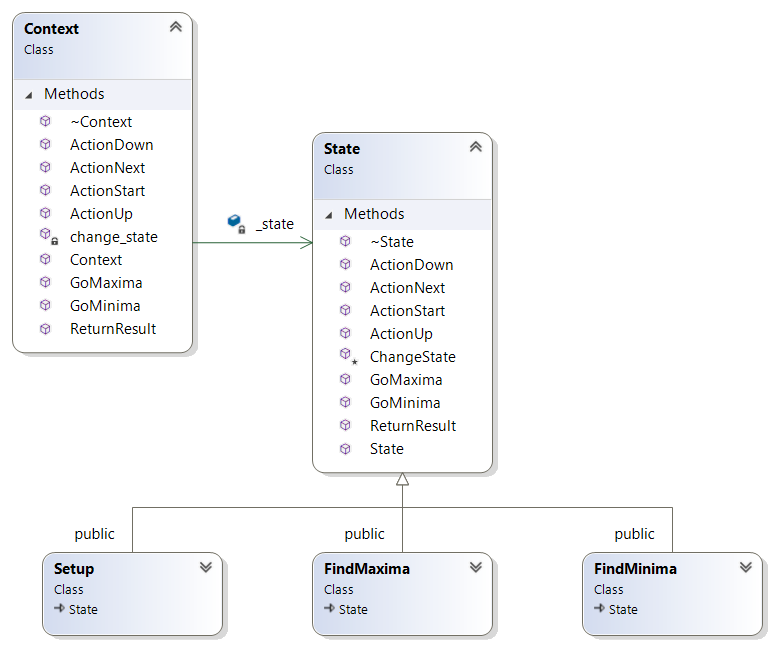
\includegraphics[width=0.7\linewidth]{diagram/StateMachine}
	\caption{An overview of the state machine and it's states.}
	\label{fig:statemachine}
\end{figure}

\subsection{GOF Singleton}
The intent of the singleton is to guarantee that a class only has one instance therefor provide a single global point of access to it. By making the class itself responsible for keeping track of its instance. The class can guarantee that no other instance can be constructed and therefore it can only have a single way access the instance.
\\
In the project the GOF Singleton, was used to keep the researcher settings so when he goes back to. It can be seen in the class diagram in Figure \ref{fig:singleton}, where the constructor is private and the only way to get access to the instance of the class is using it's instance method. This guarantees we always get the same instance returned.

\begin{figure}[h]
	\centering
	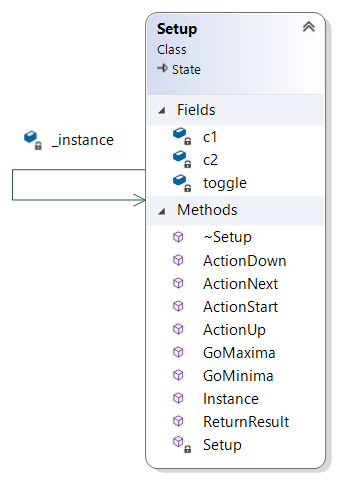
\includegraphics[width=0.4\linewidth]{diagram/singleton}
	\caption[Gof Singleton]{The setup class makes use of the Gof singleton pattern. }
	\label{fig:singleton}
\end{figure}

\subsection{GOF Command Pattern}
The intent of GOF Command Pattern is to Encapsulate a request and therefore letting one set different parameters for clients with different requests types. An example could be a message ,log requests or other requests. It has support undoable operations( operations that can't be undone ).\\

This allows software engineers to create objects that can interact with the application in a parameterize manner. The command can be stored and moved around like other objects. The main thing about this pattern is the abstract Command class which other commands inherit from. The abstract Command has a interface for executing operations hence an abstract Execute method. Concrete Command subclasses specify a Execute method with the needs for the specific Command. \\
 
In the Figure \ref{fig:commands} the commands in the PSOS is shown. The Actions are ActionDownCommand, ActionNextCommand, ActionStartCommand and ActionUpCommand. The Actions are used to change settings in the setup state and start the search for FindMinima and FindMaxima. The transitions commands are FindMaximaCommand, ReturnResultCommand and FindMinimaCommand. By using commands the code handling specific functionality are streamlined and only exist one place, hence it makes it easier to maintain and guards against code duplication.
\begin{figure}[h]
	\centering
	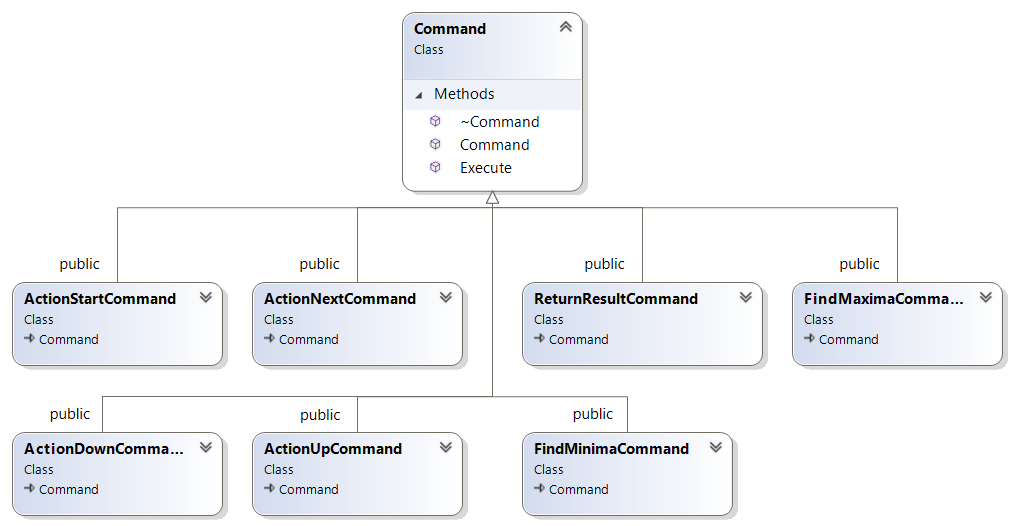
\includegraphics[width=1\linewidth]{diagram/Commands}
	\caption[The commands used to control actions and transitions]{Different Commands in the PSOS. }
	\label{fig:commands}
\end{figure}